\chapter{Granger Causality}
\label{ch-granger-c}

This chapter is based 
on the Wikipedia article 
Ref.\cite{wiki-granger-c}
and Scholarpedia article Ref.\cite{scho-granger-c}
on Granger causality and on
the book  Ref.\cite{hamilton2020time}
on time series analysis by Hamilton.

This chapter assumes the
reader has read Chapter \ref{ch-time-arma}
on the stationary time series $ARMA(p,q)$
and $VAR(p)$.

\begin{figure}[h!]
\centering
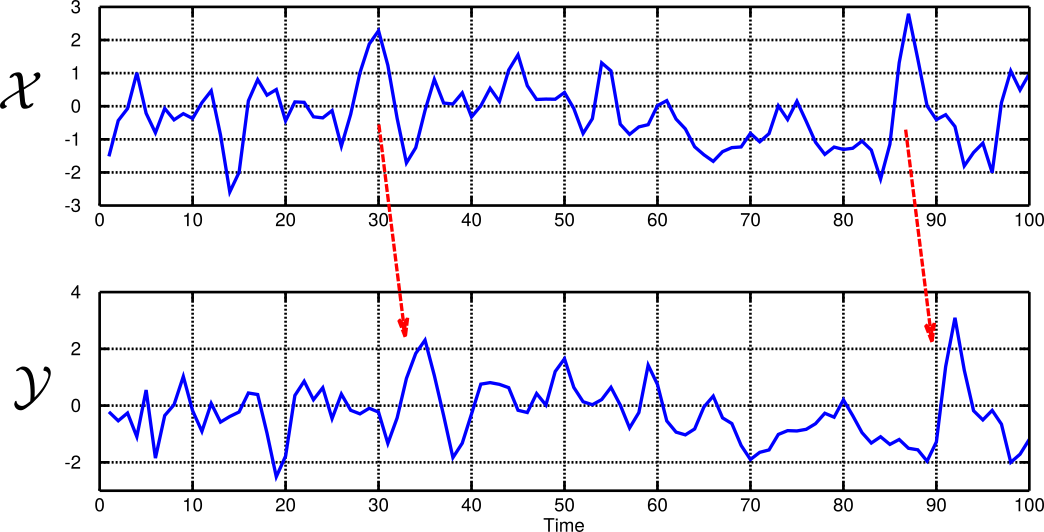
\includegraphics[width=5in]
{granger-c/g-causes.png}
\caption{When t-series $\calx$ Granger-causes
 t-series $\caly$, the patterns in 
$\calx$ are approximately repeated in $\caly$ 
after some time lag (two examples 
are indicated with arrows). Thus, 
past values of $\calx$ can be used for 
the prediction of future values of $\caly$.
(image and caption from Ref.\cite{wiki-granger-c})} 
\label{fig-g-causes}
\end{figure}

Let $\vec{\rvx}_t=[\rvx_t^{A}]_{\forall A}\in 
\RR^{nr_1\times 1}$
and
$\vec{\rvy}_t=[\rvy_t^{B}]_{\forall B}\in 
\RR^{nr_2\times 1}$.
Thus,
 $\vec{\rvx}_t$
for each $t$ is a
column vector with $nr_1$ rows,
and
$\vec{\rvy}_t$
for each $t$ is a
column vector with $nr_2$ rows.
Let $nr_1+nr_2=nr$, the total
number of rows.
Consider a vector 
t-series $\tseries{\vec{\rvx}_t, \vec{\rvy}_t}$
of type $VAR(p)$,
as defined by Eq.(\ref{eq-var-2-def}).
To simplify
the notation
of Eq.(\ref{eq-var-2-def}), we are replacing $x^1$ by $x$,
$x^2$ by $y$,
$n^1$ by $n$,
and $n^2$ by $w$.


{\renewcommand{\arraystretch}{1.5}
\beq
\left[
\begin{array}{c}
\rvx_{t}^{A}
\\
\rvy_t^{B}
\end{array}
\right]
=
\sum_{j=1}^p
\left[
\begin{array}{cc}
\alp_{j}^{\rvx|\rvx;A,A'}
&
\alp_{j}^{\rvx|\rvy;A,B'}
\\
\alp_{j}^{\rvy|\rvx;B,A'}
&
\alp_{j}^{\rvy|\rvy;B,B'}
\end{array}
\right]
\left[
\begin{array}{c}
\rvx_{t-j}^{A'}
\\
\rvy_{t-j}^{B'}
\end{array}
\right]
+
\left[
\begin{array}{c}
\rvn_{t}^{A}
\\
\rvw_{t}^{B}
\end{array}
\right]
\eeq
\label{eq-bipartite-var-q}
} 
Hence,

\beq
E_{| \vec{x}_{<t}, \vec{y}_{<t}}
\left[\rvy_{t}^{B}\right]=
\sum_{j=1}^p
\alp_j^{\rvy|\rvx;B,A'}\rvx_{t-j}^{A'}
+
\sum_{j=1}^p
\alp_j^{\rvy|\rvy;B,B'}\rvy_{t-j}^{B'}
\eeq

Let 
$\calx=\tseries{\vec{\rvx}_t}$
and
$\caly=\tseries{\vec{\rvy}_t}$.

We say {\bf $\calx$ does not G-cause
(or does not G-forecast) $\caly$},
and symbolize this by 
$ \calx\Gno \caly$, if

\beq
\alp_j^{\rvy|\rvx;B, A'}=0 \;\;\forall (j, B, A')
\eeq
or, equivalently, 
\beq
E_{| \vec{x}_{<t}, \vec{y}_{<t}}
\left[\rvy_{t}^B\right]
=
E_{| \vec{y}_{<t}}
\left[\rvy_{t}^{B}\right]\;\;\forall (B, t)
\eeq

We say {\bf $\calx$ G-causes (or G-forecasts) $\caly$}
and symbolize this by
$ \calx\Gyes \caly$, if $\calx \Gno \caly$
is false.

\begin{figure}[h!]
$$
\xymatrix{
\cdots
\vec{\rvn}_{t-3}
&\vec{\rvn}_{t-2}
&\vec{\rvn}_{t-1}
&\vec{\rvn}_t\ar[d]^1
&\vec{\rvn}_{t+1}
\cdots
\\
\cdots
\vec{\rvx}_{t-3}
&\vec{\rvx}_{t-2}\ar@/^1.7pc/[rr]^{\alp_2^{\rvx|\rvx}}
\ar@[red][ddrr]_<{\color{red}\alp_2^{\rvy|\rvx}}
&\vec{\rvx}_{t-1}\ar[r]^{\alp_1^{\rvx|\rvx}}
\ar@[red][ddr]_<{\color{red}\alp_1^{\rvy|\rvx}}
&\vec{\rvx}_t
&\vec{\rvx}_{t+1}
\cdots
\\
\\
\cdots
\vec{\rvy}_{t-3}
&\vec{\rvy}_{t-2}\ar@/_1.7pc/[rr]_{\alp^{\rvy|\rvy}_2}
\ar[uurr]^<{\alp_2^{\rvx|\rvy}}
&\vec{\rvy}_{t-1}\ar[r]_{\alp^{\rvy|\rvy}_1}
\ar[uur]^<{\alp^{\rvx|\rvy}_1}
&\vec{\rvy}_t
&\vec{\rvy}_{t+1}
\cdots
\\
\cdots
\vec{\rvw}_{t-3}
&\vec{\rvw}_{t-2}
&\vec{\rvw}_{t-1}
&\vec{\rvw}_t\ar[u]_1
&\vec{\rvw}_{t+1}
\cdots
}$$
\caption{Bnet for $VAR(2)$.
For clarity, we only
show the arrows entering
nodes $\vec{\rvx}_t$ and $\vec{\rvy}_t$.
Remove red arrows 
if $\calx$
does not G-cause $\caly$,
and
keep them if it does.
}
\label{fig-bipartite-var-2}
\end{figure}

Eq.(\ref{eq-bipartite-var-q}) describing
a bipartite $VAR(p)$
t-series can be represented by 
the bnet Fig.\ref{fig-bipartite-var-2}.
The TPMs, printed in blue,
for the two nodes $\vec{x}_t$
and $\vec{y}_t$, are as follows:


\beq\color{blue}
P(\vec{\rvx}_t|\vec{\rvx}_{[t-2, t-1]},
\vec{\rvy}_{[t-2, t-1]}, \vec{n}_{t})=
\prod_A
\indi\left(
\rvx_t^A=
\sum_{j=1}^p\alp_j^{\rvx|\rvx;A,A'}\rvx^{A'}_{t-j}
+
\sum_{j=1}^p\alp_j^{\rvx|\rvy;A,B'}\rvy^{B'}_{t-j}
+n^A_t
\right)
\eeq



\beq\color{blue}
P(\vec{\rvy}_t|\vec{\rvx}_{[t-2, t-1]},
\vec{\rvy}_{[t-2, t-1]}, \vec{w}_{t})=
\prod_B
\indi\left(
\rvy_t^B=
\sum_{j=1}^p
\underbrace{\alp_j^{\rvy|\rvx;B,A'}}
_{0?}\rvx^{A'}_{t-j}
+
\sum_{j=1}^p\alp_j^{\rvy|\rvy;B,B'}\rvy^{B'}_{t-j}
+w^B_t
\right)
\eeq

{\bf Testing for GC}

\begin{itemize}
\item
Consider the dataset

\beq
\cald=
\{(t, \vec{x}_{[t-p, t-1]},
\vec{y}_{[t-p, t-1]},
 \boxed{\vec{y}_t}):
 t\}
\eeq
Can do Linear Regression on $\cald$
with x-variables
$(\vec{x}_{[t-p, t-1]},
\vec{y}_{[t-p, t-1]})$,
y-variable 
$\vec{y}_t$,
and regression coefficients
$\alp^{\rvx|\rvx}_{[1,p]}$,
$\alp^{\rvx|\rvy}_{[1,p]}$,
$\alp^{\rvy|\rvx}_{[1,p]}$,
$\alp^{\rvy|\rvy}_{[1,p]}$.
The LR software 
yields confidence 
intervals for the
regression coefficients.
\item
Can do hypothesis testing
using the Likelihood Ratio Test\footnote{The 
Likelihood Ratio Test is 
discussed in Section
\nameref{sec-likelihood-ratio}.}

Null hypothesis $H_0: \calx\Gno \caly$ ,
Alternative hypothesis $H_1: \calx\Gyes \caly$
\item
Test for both $\calx\Gyes \caly$
and $\caly\Gyes\calx$.
\end{itemize}

{\bf Limitations}

It has been remarked that 
G-causality is not true
causality
because, even though
an event A
must precede an event B
in order to cause it,
that does not 
necessarily mean that
A causes B.
I think the 
problem 
with G-causality
is that it 
uses a bnet that
is a good fit for the data,
but not necessarily also a good {\it causal} fit
for the experiment.
One can measure the
goodness of causal fit by doing 
do-intervention
experiments (See Chapter 
\ref{ch-good-causal-fit}).
